%% Customizacoes do abnTeX2 (http://abnTeX2.googlecode.com) para o IFRS Campus Osorio v1.1
%% Por Bruno Fernandes (bruno.fernandes@osorio.ifrs.edu.br)
%% O modelo mais atualizado está disponível em bit.ly/ADSLaTeX
%%
%% abtex2-modelo-trabalho-academico.tex, v-1.9.6 laurocesar
%% Copyright 2012-2016 by abnTeX2 group at http://www.abntex.net.br/ 
%%
%% This work may be distributed and/or modified under the
%% conditions of the LaTeX Project Public License, either version 1.3
%% of this license or (at your option) any later version.
%% The latest version of this license is in
%%   http://www.latex-project.org/lppl.txt
%% and version 1.3 or later is part of all distributions of LaTeX
%% version 2005/12/01 or later.
%%
%% This work has the LPPL maintenance status `maintained'.
%% 
%% The Current Maintainer of this work is the abnTeX2 team, led
%% by Lauro César Araujo. Further information are available on 
%% http://www.abntex.net.br/
%%
%% This work consists of the files abntex2-modelo-trabalho-academico.tex,
%% abntex2-modelo-include-comandos and abntex2-modelo-references.bib
%%

% ------------------------------------------------------------------------
% ------------------------------------------------------------------------
% abnTeX2: Modelo de Trabalho Academico (tese de doutorado, dissertacao de
% mestrado e trabalhos monos em geral) em conformidade com 
% ABNT NBR 14724:2011: Informacao e documentacao - Trabalhos academicos -
% Apresentacao
% ------------------------------------------------------------------------
% ------------------------------------------------------------------------

\documentclass[
	% -- opções da classe memoir --
	12pt,				% tamanho da fonte
	openright,			% capítulos começam em pág ímpar (insere página vazia caso preciso)
	% twoside,			% para impressão em recto e verso. Oposto a oneside. FRENTE E VERSO
    oneside,			% para impressão em apenas um lado. APENAS FRENTE
	a4paper,			% tamanho do papel. 
	% -- opções da classe abntex2 --
	chapter=TITLE,		% títulos de capítulos convertidos em letras maiúsculas
	section=TITLE,		% títulos de seções convertidos em letras maiúsculas
	% -- opções do pacote babel --
	english,			% idioma adicional para hifenização
	french,				% idioma adicional para hifenização
	spanish,			% idioma adicional para hifenização
	brazil				% o último idioma é o principal do documento
	]{abntex2}


\usepackage{customizacoes-ifrs-osorio}

% ---
% Pacotes básicos 
% ---
\usepackage{tgtermes}		
\usepackage[T1]{fontenc}		% Selecao de codigos de fonte.
\usepackage[utf8]{inputenc}		% Codificacao do documento (conversão automática dos acentos)
\usepackage{lastpage}			% Usado pela Ficha catalográfica
\usepackage{indentfirst}		% Indenta o primeiro parágrafo de cada seção.
\usepackage{color}				% Controle das cores
\usepackage{graphicx}			% Inclusão de gráficos
\usepackage{microtype} 			% para melhorias de justificação
\renewcommand{\ABNTEXchapterfont}{\fontfamily{ptm}\fontseries{sbc}\selectfont}
% ---

% ----------------------------------------------
% Configuração das fontes
% ----------------------------------------------
% Algumas configurações de fontes para capitulos e seções
\renewcommand{\ABNTEXchapterfontsize}{\normalsize\bfseries}
\renewcommand{\ABNTEXpartfontsize}{\ABNTEXchapterfontsize}
\renewcommand{\ABNTEXsectionfontsize}{\normalsize}
\renewcommand{\ABNTEXsubsectionfontsize}{\normalsize\bfseries}
\renewcommand{\ABNTEXsubsubsectionfont}{\slshape\bfseries}
\renewcommand{\ABNTEXsubsubsubsectionfont}{\slshape}

% ---
% Pacotes adicionais, usados apenas no âmbito do Modelo Canônico do abnteX2
% ---
\usepackage{lipsum}				% para geração de dummy text
% ---

%pacote para inserir blocos de código
\usepackage{listings}
\usepackage{color}

\usepackage{textcomp}

\usepackage[font=small]{caption}

% ---
% Pacotes de citações
% ---
\usepackage[brazilian,hyperpageref]{backref}	 % Paginas com as citações na bibl
\usepackage[alf]{abntex2cite}	% Citações padrão ABNT


% --- 
% CONFIGURAÇÕES DE PACOTES
% --- 

%Configurações do pacote listings
%New colors defined below
\definecolor{codegreen}{rgb}{0,0.6,0}
\definecolor{codegray}{rgb}{0.5,0.5,0.5}
\definecolor{codered}{rgb}{0.8,0.1,0.3}
\definecolor{backcolour}{rgb}{0.96,0.96,0.93}

%Code listing style named "mystyle"
\lstdefinestyle{mystyle}{
	backgroundcolor=\color{backcolour},   
	commentstyle=\color{codegreen},
	keywordstyle=\bfseries\color{blue},
	numberstyle=\tiny\color{codegray},
	stringstyle=\color{codered},
	basicstyle=\footnotesize\ttfamily,
	breakatwhitespace=false,         
	breaklines=true,                 
	captionpos=t, 
	keepspaces=true,                 
	numbers=left,                    
	numbersep=5pt,
	showspaces=false,                
	showstringspaces=false,
	showtabs=false,                  
	tabsize=2,
	numberbychapter=false
}
\lstset{style=mystyle}
\renewcommand{\lstlistingname}{Código}

% ---
% Configurações do pacote backref
% Usado sem a opção hyperpageref de backref
\renewcommand{\backrefpagesname}{Citado na(s) página(s):~}
% Texto padrão antes do número das páginas
\renewcommand{\backref}{}
% Define os textos da citação
\renewcommand*{\backrefalt}[4]{
	\ifcase #1 %
		Nenhuma citação no texto.%
	\or
		Citado na página #2.%
	\else
		Citado #1 vezes nas páginas #2.%
	\fi}%
% ---

% ---
% Informações de dados para CAPA e FOLHA DE ROSTO
% ---
\titulo{Painel Pró-Mamá: reformulação do canal de comunicação do Programa Municipal de Aleitamento Materno de Osório - RS}
\autor{José Ferreira de Lima Júnior}
\local{Osório}
\data{2024}
\orientador{Bruno Fernandes}
\coorientador{} %COORIENTADOR. Deixar vazio se não houver.
\instituicao{%
  Instituto Federal de Educação, Ciência e Tecnologia do Rio Grande do Sul -- IFRS
  \par
  \textit{Campus} Osório
  \par
  Curso Superior de Tecnologia em Análise e Desenvolvimento de Sistemas}
\tipotrabalho{Trabalho de Conclusão de Curso}
% O preambulo deve conter o tipo do trabalho, o objetivo, 
% o nome da instituição e a área de concentração 
\preambulo{Trabalho de Conclusão de Curso apresentado como requisito parcial para obtenção do título de Tecnólogo em Análise e Desenvolvimento de Sistemas.}
% ---


% ---
% Configurações de aparência do PDF final

% alterando o aspecto da cor azul
\definecolor{blue}{RGB}{41,5,195}

% informações do PDF
\makeatletter
\hypersetup{
     	%pagebackref=true,
		pdftitle={\@title}, 
		pdfauthor={\@author},
    	pdfsubject={\imprimirpreambulo},
	    pdfcreator={LaTeX with abnTeX2},
		pdfkeywords={trabalho de concusão de curso}{ifrs}{campus osório}{ads}{análise e desenvolvimento de sistemas}, %adicionar as keywords do trabalho
		colorlinks=true,       		% false: boxed links; true: colored links
    	linkcolor=blue,          	% color of internal links
    	citecolor=blue,        		% color of links to bibliography
    	filecolor=magenta,      		% color of file links
		urlcolor=blue,
		bookmarksdepth=4
}
\makeatother
% --- 

% --- 
% Espaçamentos entre linhas e parágrafos 
% --- 
% O tamanho do parágrafo é dado por:
\setlength{\parindent}{1.3cm}
% Controle do espaçamento entre um parágrafo e outro:
\setlength{\parskip}{0.2cm}  % tente também \onelineskip

% ---
% compila o indice
% ---
\makeindex
% ---

% ----
% Início do documento
% ----
\begin{document}

% Seleciona o idioma do documento (conforme pacotes do babel)
%\selectlanguage{english}
\selectlanguage{brazil}

% Retira espaço extra obsoleto entre as frases.
\frenchspacing

% ----------------------------------------------------------
% ELEMENTOS PRÉ-TEXTUAIS
% ----------------------------------------------------------
% \pretextual

% ---
% Capa ((Obrigatório)
% ---
\imprimircapa
% ---

% ---
% Folha de rosto (Obrigatório)
% (o * indica que haverá a ficha bibliográfica)
% ---
\imprimirfolhaderosto*
% ---

% ---
% Inserir errata (Opcional)
% ---
%\begin{errata}

%Elemento opcional da \citeonline[4.2.1.2]{NBR14724:2011}. Exemplo:

%\vspace{\onelineskip}

FERRIGNO, C. R. A. \textbf{Tratamento de neoplasias ósseas apendiculares com
reimplantação de enxerto ósseo autólogo autoclavado associado ao plasma
rico em plaquetas}: estudo crítico na cirurgia de preservação de membro em
cães. 2011. 128 f. Tese (Livre-Docência) - Faculdade de Medicina Veterinária e
Zootecnia, Universidade de São Paulo, São Paulo, 2011.

\begin{table}[htb]
\center
\footnotesize
\begin{tabular}{|p{1.4cm}|p{1cm}|p{3cm}|p{3cm}|}
  \hline
   \textbf{Folha} & \textbf{Linha}  & \textbf{Onde se lê}  & \textbf{Leia-se}  \\
    \hline
    1 & 10 & auto-conclavo & autoconclavo\\
   \hline
\end{tabular}
\end{table}

\end{errata}
% ---

% ---
% Inserir folha de aprovação (Obrigatório)
% ---
% Isto é um exemplo de Folha de aprovação, elemento obrigatório da NBR
% 14724/2011 (seção 4.2.1.3).
%
\begin{folhadeaprovacao}

  \begin{center}
    {\ABNTEXchapterfont\large\imprimirautor}

    \vspace*{\fill}\vspace*{\fill}
    \begin{center}
      \ABNTEXchapterfont\bfseries\Large\imprimirtitulo
    \end{center}
    \vspace*{\fill}
    
    \hspace{.45\textwidth}
    \begin{minipage}{.5\textwidth}
        \imprimirpreambulo
    \end{minipage}%
    \vspace*{\fill}
   \end{center}
     
   %Adicionar o texto abaixo depois do trabalho ser aprovado pela banca.   
   %Trabalho aprovado. \imprimirlocal, xx de xxxxxxxxx de 201X:

   \assinatura{\textbf{\imprimirorientador} \\ Orientador} 
   \assinatura{\textbf{Professor} \\ Convidado 1}
   \assinatura{\textbf{Professor} \\ Convidado 2}
   %\assinatura{\textbf{Professor} \\ Convidado 3}
   %\assinatura{\textbf{Professor} \\ Convidado 4}
    
    \vspace*{1.5cm}
   \begin{center}
    \vspace*{0.5cm}
    {\large\imprimirlocal}
    \par
    {\large\imprimirdata}
    \vspace*{1cm}
  \end{center}
  
\end{folhadeaprovacao}
% ---

% ---
% Dedicatória (Opcional)
% ---
%\begin{dedicatoria}
   \vspace*{\fill}
   \centering
   \noindent
   \textit{ Este trabalho é dedicado a...} \vspace*{\fill}
\end{dedicatoria}
% ---

% ---
% Agradecimentos (Opcional)
% ---
% \begin{agradecimentos}
Os agradecimentos principais são direcionados à Gerald Weber, Miguel Frasson,
Leslie H. Watter, Bruno Parente Lima, Flávio de Vasconcellos Corrêa, Otavio Real
Salvador, Renato Machnievscz\footnote{Os nomes dos integrantes do primeiro
projeto abn\TeX\ foram extraídos de
\url{http://codigolivre.org.br/projects/abntex/}} e todos aqueles que
contribuíram para que a produção de trabalhos acadêmicos conforme
as normas ABNT com \LaTeX\ fosse possível.

Agradecimentos especiais são direcionados ao Centro de Pesquisa em Arquitetura
da Informação\footnote{\url{http://www.cpai.unb.br/}} da Universidade de
Brasília (CPAI), ao grupo de usuários
\emph{latex-br}\footnote{\url{http://groups.google.com/group/latex-br}} e aos
novos voluntários do grupo
\emph{\abnTeX}\footnote{\url{http://groups.google.com/group/abntex2} e
\url{http://www.abntex.net.br/}}~que contribuíram e que ainda
contribuirão para a evolução do \abnTeX.

\end{agradecimentos}
% ---

% ---
% Epígrafe (Opcional)
% ---
%\begin{epigrafe}
    \vspace*{\fill}
	\begin{flushright}
		\textit{``Não vos amoldeis às estruturas deste mundo, \\
		mas transformai-vos pela renovação da mente, \\
		a fim de distinguir qual é a vontade de Deus: \\
		o que é bom, o que Lhe é agradável, o que é perfeito.\\
		(Bíblia Sagrada, Romanos 12, 2)}
	\end{flushright}
\end{epigrafe}

% ---

% ---
% RESUMOS
% ---

% resumo em português (Obrigatório)
\setlength{\absparsep}{18pt} % ajusta o espaçamento dos parágrafos do resumo
\begin{resumo}
	Segundo a \citeonline[3.1-3.2]{NBR6028:2003}, o resumo deve ressaltar o
	objetivo, o método, os resultados e as conclusões do documento. A ordem e a extensão
	destes itens dependem do tipo de resumo (informativo ou indicativo) e do
	tratamento que cada item recebe no documento original. O resumo deve ser
	precedido da referência do documento, com exceção do resumo inserido no
	próprio documento. (\ldots) As palavras-chave devem figurar logo abaixo do
	resumo, antecedidas da expressão Palavras-chave:, separadas entre si por
	ponto e finalizadas também por ponto.
	
	\textbf{Palavras-chave}: latex. abntex. editoração de texto.  %alterar para as palavras-chave do trabalho
\end{resumo}

% resumo em inglês (Obrigatório)
\begin{resumo}[Abstract]
 \begin{otherlanguage*}{english}
   This is the english abstract.

   \vspace{\onelineskip}
 
   \noindent 
   \textbf{Keywords}: latex. abntex. text editoration. %alterar para as palavras-chave do trabalho
 \end{otherlanguage*}
\end{resumo}

% resumo em francês (Opcional)
%\begin{resumo}[Résumé]
 \begin{otherlanguage*}{french}
    Il s'agit d'un résumé en français.
 
   \textbf{Mots-clés}: latex. abntex. publication de textes.  %alterar para as palavras-chave do trabalho
 \end{otherlanguage*}
\end{resumo}

% resumo em espanhol (Opcional)
%\begin{resumo}[Resumen]
 \begin{otherlanguage*}{spanish}
   Este es el resumen en español.
  
   \textbf{Palabras clave}: latex. abntex. publicación de textos. %alterar para as palavras-chave do trabalho
 \end{otherlanguage*}
\end{resumo}

% ---

% ---
% inserir lista de ilustrações (Opcional)
% ---
% \pdfbookmark[0]{\listfigurename}{lof}
% \listoffigures*
% \cleardoublepage
% ---

% ---
% inserir lista de tabelas (Opcional)
% ---
% \pdfbookmark[0]{\listtablename}{lot}
% \listoftables*
% \cleardoublepage
% ---

% ---
% inserir lista de abreviaturas e siglas (Opcional)
% ---
% \begin{siglas}
  \item[ABNT] Associação Brasileira de Normas Técnicas
  \item[abnTeX] ABsurdas Normas para TeX
\end{siglas}
% ---

% ---
% inserir lista de símbolos (Opcional)
% ---
%\begin{simbolos}
  \item[$ \Gamma $] Letra grega Gama
  \item[$ \Lambda $] Lambda
  \item[$ \zeta $] Letra grega minúscula zeta
  \item[$ \in $] Pertence
\end{simbolos}
% ---

% ---
% inserir o sumario (Obrigatório)
% ---
\pdfbookmark[0]{\contentsname}{toc}
\tableofcontents*
\cleardoublepage
% ---


% ----------------------------------------------------------
% ELEMENTOS TEXTUAIS
% ----------------------------------------------------------
\textual

% ----------------------------------------------------------
% Introdução (Obrigatório)
% ----------------------------------------------------------
% ----------------------------------------------------------
% Introdução (com numeração)
% ----------------------------------------------------------
\chapter{Introdução}
% ----------------------------------------------------------

A amamentação é a primeira e mais importante contribuição que toda mãe pode dar à saúde do seu filho, assim como à sua própria saúde. No entanto, apesar dos esforços contínuos da Organização Mundial de Saúde em fundamentar pilares para disseminação de informações e recomendações, ainda enfrentamos desafios significativos na promoção e apoio ao aleitamento materno.

Segundo a OMS \citeonline{oms9241561300}, as autoridades competentes devem implementar medidas sociais para dar suporte e proteção às gestantes e mães. Isso implica em manter as mulheres adequadamente informadas sobre assuntos relacionados à alimentação infantil, que recebam suporte apropriado da família e comunidade a fim de facilitar e encorajar a amamentação, inibindo quaisquer influências contrárias.

Neste contexto, a partir da parceria entre o programa municipal de aleitamento materno da secretaria de saúde de Osório e o IFRS Campus Osório, foi criado o aplicativo Pró-Mamá e seu respectivo painel administrativo para controle dos servidores públicos.O \emph{app} foi lançado em agosto de 2018 e na época estava disponível para \emph{download} na \emph{play store} e \emph{app store}, qualquer usuário, mas principalmente as mães podiam acessar e obter informações sobre o aleitamento materno, registrar dúvidas e acompanhar os marcos do desenvolvimento de seu bebê.

Apesar do seu sucesso, de acordo com o \citeonline{promamapremiacao} o aplicativo conquistou o 1º lugar na categoria “Atenção Básica” no 31º Congresso do Conselho das Secretarias Municipais de Saúde do Rio Grande do Sul (Cosems/RS), atualmente encontra-se em estado defasado e em inconformidade com a Lei Geral de Proteção de Dados (LGPD), o que ocasionou na remoção do aplicativo nas lojas dos dispositivos móveis.

O presente trabalho tem como objetivo reestruturar o Painel Pró-Mamá para atender as necessidades das leis de privacidade de dados dos usuários e suas restrições de segurança, além de implantar novas tecnologias para facilitar o suporte de forma eficiente e segura no futuro. Dessa forma, não só contribuindo para manter as funcionalidades já estabelecidas, mas também agregar com novas soluções propostas pelos próprios servidores ao longo da observação do uso do painel desde seu lançamento.

\section{OBJETIVOS}

\subsection{Objetivo geral}

Reconstrução do painel e adição de novas funcionalidades…

\subsection{Objetivos específicos}

\begin{itemize}
  \item Analisar os requisitos funcionais, não-funcionais e regras de negócio do Painel Pró-Mamá;
  \item Planejar arquitetura do painel administrativo e API;
  \item Estruturar banco de dados e operação para migração dos dados retroativos;
  \item Desenvolver painel e API;
  \item Manutenção e adição de novas funcionalidades para o sistema.
\end{itemize}

\section{JUSTIFICATIVA}

Importância da tecnologia em prol da saúde no aleitamento materno citação OMS…
Trazer resultados do programa e a necessidade que se perpetue…

% ---


% ----------------------------------------------------------
% Desenvolvimento (Obrigatório)
% ----------------------------------------------------------
% ---
% Capitulo 1
% ---
\chapter{Referencial Teórico}\label{cap_exemplos}

% ---

% ---
% Capitulo 2
% ---
\chapter{Trabalhos Relacionados}\label{cap_exemplos}

A presente pesquisa foi realizada a partir do levantamento de informações sobre os principais sistemas gerenciadores de conteúdo do mercado. Pretende-se classificá-los a partir de sua quota de mercado, popularidade e características semelhantes aos requisitos necessários ao Painel Pró-Mamá. Por fim, serão selecionados três, de acordo com alguns critérios, para um detalhamento a fim de elucidar as principais funcionalidades, vantagens/desvantagens e sua portabilidade para construção de um painel administrativo.

\section{Pesquisa de mercado}

Foi utilizado como base a pesquisa realizada pela \citeonline{w3techs_cms}, uma organização responsável por monitorar e analisar diversas tecnologias na internet. Em seus estudos buscou-se a análise da presença de mercado dos CMS na publicação de websites. No gráfico abaixo pode-se analisar duas barras, em vermelho representam sites criados com sistema gerenciador de conteúdo e em azul sites com dados estáticos.

\begin{figure}[htb]
  \caption{\label{fig_grafico} Quota de mercado dos CMS}
  \begin{center}
    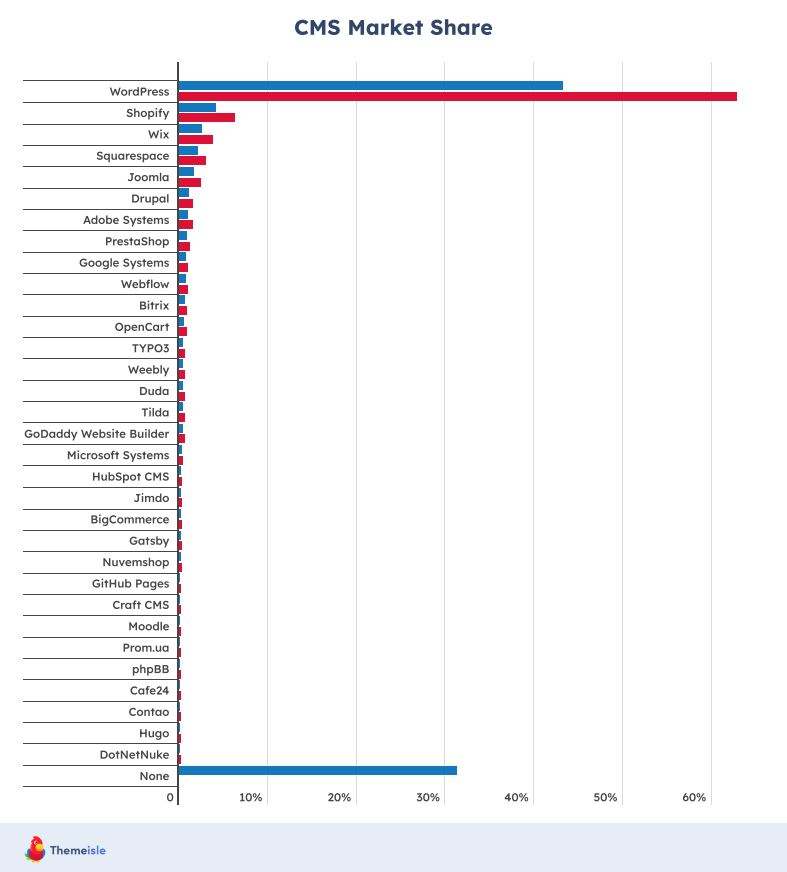
\includegraphics[scale=0.45]{imagens/w3techs-cms.JPG}
  \end{center}
  \legend{Fonte: \citeonline{themeisle_cms_market_share}}
\end{figure}

Atualmente cerca de 69\% dos sites na internet foram criados a partir de um CMS, dessa parcela, somente o WordPress detém de aproximadamente 43\% de todos os websites. Apesar da predominância do WordPress, destacam-se também a plataforma Wix e Shopify que vem logo em seguida no ranking.

\section{Detalhamento}

Dado os CMS mencionados, serão traçadas informações e detalhes a seu respeito nesta seção.

\subsection{WordPress}

O \citeonline{wordpress} é uma plataforma CMS de código aberto utilizada na criação de cerca de 43\% de todos os websites presentes na internet. Sua configuração em muitos serviços de hospedagem, como a HostGator, pode ser solicitada em conjunto com o plano selecionado, bastando apenas alterar seu domínio para redirecionar para o servidor. No caso da instalação manual é preciso atender aos requisitos: PHP v7.4 ou superior, MySQL v5.7 / MariaDB v10.3 ou superior e suporte HTTPS, para assim transferir via FTP o sistema e instalá–lo em conjunto com a base de dados.

Uma de suas principais vantagens é o painel de edição que permite com que sejam construídas interfaces a partir de temas disponibilizados pela comunidade. Nesta seção de aparência há dois temas iniciais, porém também encontra-se um repositório com milhares, alguns pagos e outros gratuitos. Apesar de ser um software livre, o intuito do produto é que sejam comercializados plugins para que o dono do site consiga adicionar as funcionalidades desejadas.

No mesmo local do editor outros usuários podem acessar para gerenciar o conteúdo do site, assim o WordPress permite com que sejam designados papéis para controle de quem pode editar a estrutura ou somente o texto de espaços pré-definidos por outro administrador.

Além de acessar por navegador web, o WordPress possui seu aplicativo disponível nas lojas para que o administrador possa gerenciar seu site a partir de seu dispositivo móvel.

\subsection{Wix}

\citeonline{wix} é a plataforma paga para criação e gerenciamento de conteúdo de sites que mais se popularizou nos últimos tempos, seguida de WordPress e Shopify. Sua quota de mercado cresceu em torno de 800\% entre 2016 e 2023. Criada em 2006, seu objetivo é simplificar a publicação de websites sem a necessidade de conhecimento prévio.

Não há necessidade de instalar ou contratar um serviço de hospedagem, basta conectar seu domínio e configurar um tema para que já se possa visualizar o site em construção. Seus templates vão desde: blog, landing page, portfólio, marketplace, anúncios, etc.

Uma de suas principais funcionalidades é o editor com tecnologia arrasta e solta, a qual permite com que o administrador mova os elementos do site da maneira que quiser. Cada elemento de design é personalizável, sendo possível redimensionar, recolorir, girar e alinhar até atingir a forma desejada.

Outra aposta está em sua ferramenta de inteligência artificial Wix ADI, onde algumas perguntas são feitas e a partir delas um site com conteúdo e imagens integradas é criado. Durante as etapas é possível personalizar a paleta de cores, logo, design e assim o restante é construído de forma personalizada as regras de negócios identificadas pelo usuário.

Assim como o WordPress, o aplicativo Wix Owner também é designado para gerenciar o site, possui funcionalidades como: edição e compartilhamento de posts, aceitação de reservas e pagamentos, conversa pelo chat com visitantes, etc. A ideia é que o dono do site possa acessar seu portal tanto a partir do navegador web, quanto pelo seu dispositivo móvel.

\subsection{Shopify}

\citeonline{shopify} é uma plataforma de e-commerce lançada em 2006 que permite a indivíduos e empresas criarem suas próprias lojas onlines. Atrás somente do WordPress, é o segundo CMS mais popular do mercado, só nos Estados Unidos são mais de dois milhões e meio de comércios eletrônicos publicados.

Assim como o Wix, não é necessário instalá-lo, uma vez conectado ao domínio é possível visualizar a loja na internet. Como um sistema líder na temática de varejo, seus templates seguem os modelos de lojas virtuais, com listagem de produtos e páginas de checkout. Há também a possibilidade de criar blogs pessoais e landing pages, porém qualquer personalização que vá além deve ser feita manualmente pelo editor.

Por tratar de marketplaces, sua infraestrutura é robusta e confiável, o que garante boa velocidade de carregamento das páginas e alta confiabilidade. Além de suporte 24/7 via chat em qualquer plano contratado.

Seus recursos se assemelham aos plugins do WordPress, nesse caso na loja aplicativos podem ser configurados para adicionar as funcionalidades, há desde: gestão de inventário, análise de dados, marketing, gateway de pagamentos, tudo que um comércio precisa.

\section{Comparações}

Dentre os sistemas analisados, dado que seu uso é genérico, ou seja, são ferramentas que permitem a criação de: blogs, comércios digitais, landing page, etc. Será comparado a partir do viés de sua utilização em painéis administrativos e como o conteúdo é distribuído para não só o site na web, mas sim para dispositivos móveis. Por isso, os três CMS possuem uma condição inicial em comum que é a possibilidade de acesso do dado via API Rest, assim a aplicação móvel pode fazer solicitações HTTP para consumir e atuar em cima das entidades.

Algumas tabelas serão apresentadas para que sejam vistos os comparativos produzidos:

\begin{table}[htb]
  \begin{center}
    \ABNTEXfontereduzida
    \caption{comparações entre os sistemas selecionados.}
    \label{tab-comparacao-1}
    \begin{tabular}{c|c|c|c}
      %\hline
      \phantom{.}     & \textbf{Tema administrativo} & \textbf{Design responsivo} & \textbf{Gratuito} \\
      \hline
      WordPress       & X                            & X                          &
      X                                                                                               \\
      \hline
      Wix             & \phantom{.}                  &
      X               & \phantom{.}                                                                   \\
      \hline
      Shopify         & \phantom{.}                  & X                          & \phantom{.}       \\
      \hline
      Painel Pró-Mamá & X                            & X                          & X                 \\
      % \hline
    \end{tabular}
    \legend{Fonte: autor.}
  \end{center}
\end{table}

Conforme as informações acima da \autoref{tab-comparacao-1}, pode-se observar que além do WordPress que é líder de mercado, apenas o Painel Pró-Mamá oferece tema administrativo de forma gratuita e com estilização responsiva.

\begin{table}[htb]
  \begin{center}
    \ABNTEXfontereduzida
    \caption{comparações entre os sistemas selecionados.}
    \label{tab-comparacao-2}
    \begin{tabular}{c|c|c}
      %\hline
      \phantom{.}     & \textbf{Enviar e-mail} & \textbf{\emph{Push notification}} \\
      \hline
      WordPress       & X                      & X*                                \\
      \hline
      Wix             & X                      &
      X*                                                                           \\
      \hline
      Shopify         & X                      & \phantom{.}                       \\
      \hline
      Painel Pró-Mamá & X                      & X                                 \\
      % \hline
    \end{tabular}
    \legend{Fonte: autor.}
  \end{center}
\end{table}

A partir da \autoref{tab-comparacao-2}, como a maioria das ferramentas de mercado, todas implementam o envio de e-mail para seus usuários. Porém, somente WordPress e Wix tem em suas lojas plugins para Push Notification, entretanto este somente funciona para o site web, ao contrário do que o Painel Pró-Mamá oferece que é o envio da notificação para os usuários do aplicativo nos dispositivos móveis.

\begin{table}[htb]
  \begin{center}
    \ABNTEXfontereduzida
    \caption{comparações entre os sistemas selecionados.}
    \label{tab-comparacao-3}
    \begin{tabularx}{\textwidth}{|c|>{\centering\arraybackslash}X|>{\centering\arraybackslash}X|>{\centering\arraybackslash}X|>{\centering\arraybackslash}X|>{\centering\arraybackslash}X|}
      %\hline
      \phantom{.}     & \textbf{Facilidade uso usuário não técnico} & \textbf{Gráfico e estatísticas} & \textbf{CRUD de dados} & \textbf{Envio de arquivos} & \textbf{Exportação de dados em diferentes formatos} \\
      \hline
      WordPress       & \phantom{.}                                 & X                               &
      X               & X                                           & \phantom{.}                                                                                                                                 \\
      \hline
      Wix             & X                                           &
      X               & X                                           & X                               & \phantom{.}                                                                                               \\
      \hline
      Shopify         & X                                           & X                               & X                      & X                          & \phantom{.}                                         \\
      \hline
      Painel Pró-Mamá & X                                           & X                               & X                      & X                          & X                                                   \\
      % \hline
    \end{tabularx}
    \legend{Fonte: autor.}
  \end{center}
\end{table}

Observa-se na \autoref{tab-comparacao-3} que assim como todos os CMS, o Painel Pró-Mamá também possibilita a manipulação e visualização dos dados, sendo texto ou arquivo. Porém dentre os sistemas gratuitos, é o único que se preocupa com o uso por usuário não técnico, haja vista que tratam-se dos servidores públicos do projeto Pró-Mamá.

Outro ponto interessante do Painel Pró-Mamá é a capacidade de exportar os dados nos formatos auxiliares a sistemas da secretaria de saúde do município de Osório, facilitando assim o cadastro das mães pelos profissionais responsáveis.

% ---

% ---
% Capitulo 3
% ---
\chapter{Metodologia}

% ---

% ---
% Capitulo 4
% ---
\chapter{Desenvolvimento}

% ---

% ---
% Conclusão
% ---
\chapter{Conclusão}
% ---

% ---


% ----------------------------------------------------------
% ELEMENTOS PÓS-TEXTUAIS
% ----------------------------------------------------------
\postextual
% ----------------------------------------------------------

% ----------------------------------------------------------
% Referências bibliográficas (Obrigatório)
% ----------------------------------------------------------
\bibliography{elementos-pos-textuais/referencias}


% ----------------------------------------------------------
% Glossário (Opcional)
% ----------------------------------------------------------
%
% Consulte o manual da classe abntex2 para orientações sobre o glossário.
%
%\glossary


% ----------------------------------------------------------
% Apêndices (Opcional)
% ----------------------------------------------------------
% ---
% Inicia os apêndices
% ---
% \begin{apendicesenv}

% % ----------------------------------------------------------
\chapter{Quisque libero justo}
% ----------------------------------------------------------

\lipsum[50]
% % ----------------------------------------------------------
\chapter{Nullam elementum urna vel imperdiet sodales elit ipsum pharetra ligula
ac pretium ante justo a nulla curabitur tristique arcu eu metus}
% ----------------------------------------------------------
\lipsum[55-57]

% \end{apendicesenv}
% ---


% ----------------------------------------------------------
% Anexos (Opcional)
% ----------------------------------------------------------
% ---
% Inicia os anexos
% ---
% \begin{anexosenv}

% % ---
\chapter{Morbi ultrices rutrum lorem.}
% ---
\lipsum[30]
% % ---
\chapter{Cras non urna sed feugiat cum sociis natoque penatibus et magnis dis
parturient montes nascetur ridiculus mus}
% ---

\lipsum[31]
% % ---
\chapter{Fusce facilisis lacinia dui}
% ---

\lipsum[32]

% \end{anexosenv}


%---------------------------------------------------------------------
% INDICE REMISSIVO (Opcional)
%---------------------------------------------------------------------
%\phantompart
%\printindex
%---------------------------------------------------------------------

\end{document}
